\newpage
\appendix
\onecolumn
\large
\begin{center}
   \emph{Appendix of paper ``Decision Mamba: Reinforcement Learning via Hybrid Selective Sequence Modeling"} 
\end{center} 
\normalsize

\section{Pseudocode of Decision Mamba-Hybrid}
\label{appendix A}

\begin{algorithm}[h!]
\caption{Decision Mamba-Hybrid.}
\label{DM-H algorithm}
\LinesNumbered
\KwIn{A dataset of Trajectories, Max Iterations $M$ as training phase, Max episodes $m$ at testing phase, A number of trajectories $n$ in across-episodic contexts used in Mamba model, A number of steps of actions $c$ for one sub-goals}
\KwOut{The generated actions}
\textbf{//Training} \\
\For{$i=1$ $\textbf{to}$ $M$}{
    Randomly sample $n$ episodes from dataset $s=(\tau^{1},\tau^{2},\dots,\tau^{n})$ \\
    Sort $n$ episodes ascending according to their returns $\sum_{t=0}^T{r_t^1}\leq\sum_{t=0}^T{r_t^2}\leq\dots\leq\sum_{t=0}^T{r_t^n}$ \\
    Concatenate $n$ episodes as a across-episodic context $s_h=(\tau_m^{1},\tau_m^{2},\dots,\tau_m^{n})$ based on Equation~\eqref{mamba} \\
    Mamba module predicts the next sub-goals tokens from the across-episodic context \\
    Build a local short-term sequence every $c$ steps based on Equation~\eqref{transformer} \\
    Select the high-value states from the offline data based on the weighted average of accumulated rewards $\sum_{t=i+1}^jr_k/(j-i)$
    Build a similar local short-term sequence every $c$ steps based on Equation~\eqref{g_transformer}\\
    The transformer module predicts the next $c$ steps action tokens for each predicted sub-goals token from Mamba and selected high-value sub-goals \\
    Train Mamba and transformer models based on the loss of predicted actions end-to-end \\
}    
\textbf{//Testing} \\
\For{$i=1$ $\textbf{to}$ $m$}{
    Start a new episode $i$ and reset the timestep $t=0$ \\
    \While{$t\leq T$}{
        Mamba model generates next sub-goal token $\textbf{z}_t^i$ based on the historical trajectories $(\tau_m^{1},\tau_m^{2},\tau_m^{i-1},\dots,s_t^i)$, where $\tau_m^{i}$ is expressed as Equation~\eqref{mamba} \\
        \For{$k=0$ $\textbf{to}$ $c-1$}{
            The transformer model generates next action $a_{t+k}^i$ based on the local context $(\textbf{z}_t^i,s_t^i,a_t^i,r_t^i,\dots,\textbf{z}_{t}^i,s_{t+k}^i)$ \\
        }
        Compute the sum of $c$ steps rewards $\hat{r}_t^i=\sum_{k=t}^{t+c-1}{r_k^i}$ \\
        Receive the next observation or state $s_{t+c}^i$ \\
        Update the across-episodic context $(\tau_m^{1},\tau_m^{2},\tau_m^{i-1},\dots,s_t^i,\textbf{z}_t^i,\hat{r}_t^i,d_t^i,s_{t+c}^i)$ \\
        Update time step $t = t+c$ \\
    }
}
\end{algorithm}

In Algorithm~\ref{DM-H algorithm}, we introduce the training and testing process of DM-H. At each iteration, we first construct a long-term sequence consisting of multiple trajectories, as described in lines 3-5. Mamba model predicts sub-goals based on the long-term sequence (line 6). Then, each sub-goal will correspond to a short sequence of $c$ steps actions, as described in line 7. 
To encourage the transformer to rely on Mamba's predictions, we select the high-value states from the offline data and transform them into sub-goals to reconstruct another short sequence of $c$ steps actions (line 8). Based on the short sequence and reconstructed sequences, the transformer model predicts $c$ steps actions (line 9). Finally, the predicted actions are evaluated with either cross-entropy loss or mean-squared error, depending on whether the actions are discrete or continuous. The losses from each time step are averaged and updated in all models end-to-end, as described in line 10.


\begin{table}[t]
\centering
\caption{Hyperparameters of DM-H.}
\resizebox{0.95\textwidth}{!}{
\begin{tabular}{@{}l|l|l@{}}
\toprule
 & Hyperparameters & Value \\ \midrule
\multirow{4}{*}{Mamba} & Number of layers & 2 \\
 & Embedding dimension & 128 \\
 & Expand factor & 2 \\
 & Convolution size & 4\\  \midrule
\multirow{6}{*}{Transformer} & Number of layers & 3 \\
 & Number of attention heads & 3 \\
 & Embedding dimension & 128 \\
 & Activation function & ReLU \\ 
 & $c$ steps controlled by one sub-goal & 20 D4RL and Large Grid World \\
 &  & 5 Grid World and Tmaze\\ \midrule
\multirow{7}{*}{Training}& Batch size & 128 \\
 & Dropout & 0.1 \\
 & Learning rate & 1e-4 \\
 & Learning rate decay & Linear warmup for 1e5 steps \\ 
 & Grad norm clip & 0.25 \\
 & Weight decay & 1e-4 \\
 & Number of trajectories to form across-episodic contexts $n$ & 4 (Large) Dark Key-to-Door \\
 &  & 10 other tasks in Grid World \\
 &  & 4 D4RL \\ \midrule
\multirow{14}{*}{Testing} & Target return for Tmaze & 1 \\
 & Target return for HalfCheetah & 12000 \\
 & Target return for Hopper & 3600 \\
 & Target return for Walker & 5000 \\
 & Target return for Darkroom & 20 \\
 & Target return for Darkroom Hard & 1 \\
 & Target return for Darkroom Key-to-Door & 2 \\
 & Target return for Large Darkroom & 15 \\
 & Target return for Large Darkroom Hard & 1 \\
 & Target return for Large Darkroom Key-to-Door & 2 \\
 & Number of trajectories to form across-episodic contexts $n$ & 4 (Large) Dark Key-to-Door \\
 &  & 10 other tasks in Grid World \\
 &  & 4 D4RL \\ 
 \bottomrule
\end{tabular}
}
\label{hyper}
\end{table}


During online testing, DM-H needs to generate actions autoregressively and interact with the environment in $m$ episodes. At step $t$ of episode $i$ (line 16), Mamba module first generates a sub-goal token $\textbf{z}_t^i$ conditioned on the historical context $(\tau_m^{1},\tau_m^{2},\tau_m^{i-1},\dots,s_t^i)$, where $\tau_m^{i}$ is expressed as Equation~\eqref{mamba}. Then, the transformer will generate the following $c$ steps actions $(a_t,\dots,a_{t+c-1})$ autoregressively, as described in lines 17-19. Finally, we update the across-episodic context for generating the next sub-goal $\textbf{z}_{t+c}^i$, as described in lines 20-23.

\section{Experimental Details}
\label{appendix B}

Source code is available at 
\href{https://github.com/SiliHuang-ai/hybrid_mamba}{here}.
% \href{https://anonymous.4open.science/r/hybrid_decision_mamba-3B84}{here}.

\noindent\textbf{Dataset: Grid World.}~~
The evaluation environments of Grid World provide a 2D discrete POMDP where an agent spawns in a room and must find a goal location. The agent only observes its own $(x,y)$ coordinates but does not know the goal location, which is required to deduce it from the rewards received. The room dimensions are $9\times9$ with the agent's possible actions, including moving one step either left, right, up, down, or staying idle. In Darkroom, an episode lasts 20 steps, and the agent can obtain a reward ($r=1$) each time the goal is achieved. The Darkroom Hard is a variant of Darkroom. In the Darkroom Hard, agents only obtain a reward when the goal is achieved first. In the Dark Key-to-Door, the length of an episode is 50, where the agent is required to locate an invisible key to receive a one-time reward first and then identify an invisible door to obtain another one-time reward. In addition, we create a long-term variant of Large Darkroom, Large Darkroom Hard, and Large Darkroom Key-to-Door, where the coordinate space of each environment is expanded to $40\times40$, and the episode length is expanded 10 times. 

\setlength{\belowcaptionskip}{-0.0cm} %调整图片标题与下文距离 
\setlength{\abovecaptionskip}{-0.0cm} %调整图片标题与图距离
\begin{figure*}
    \centering
    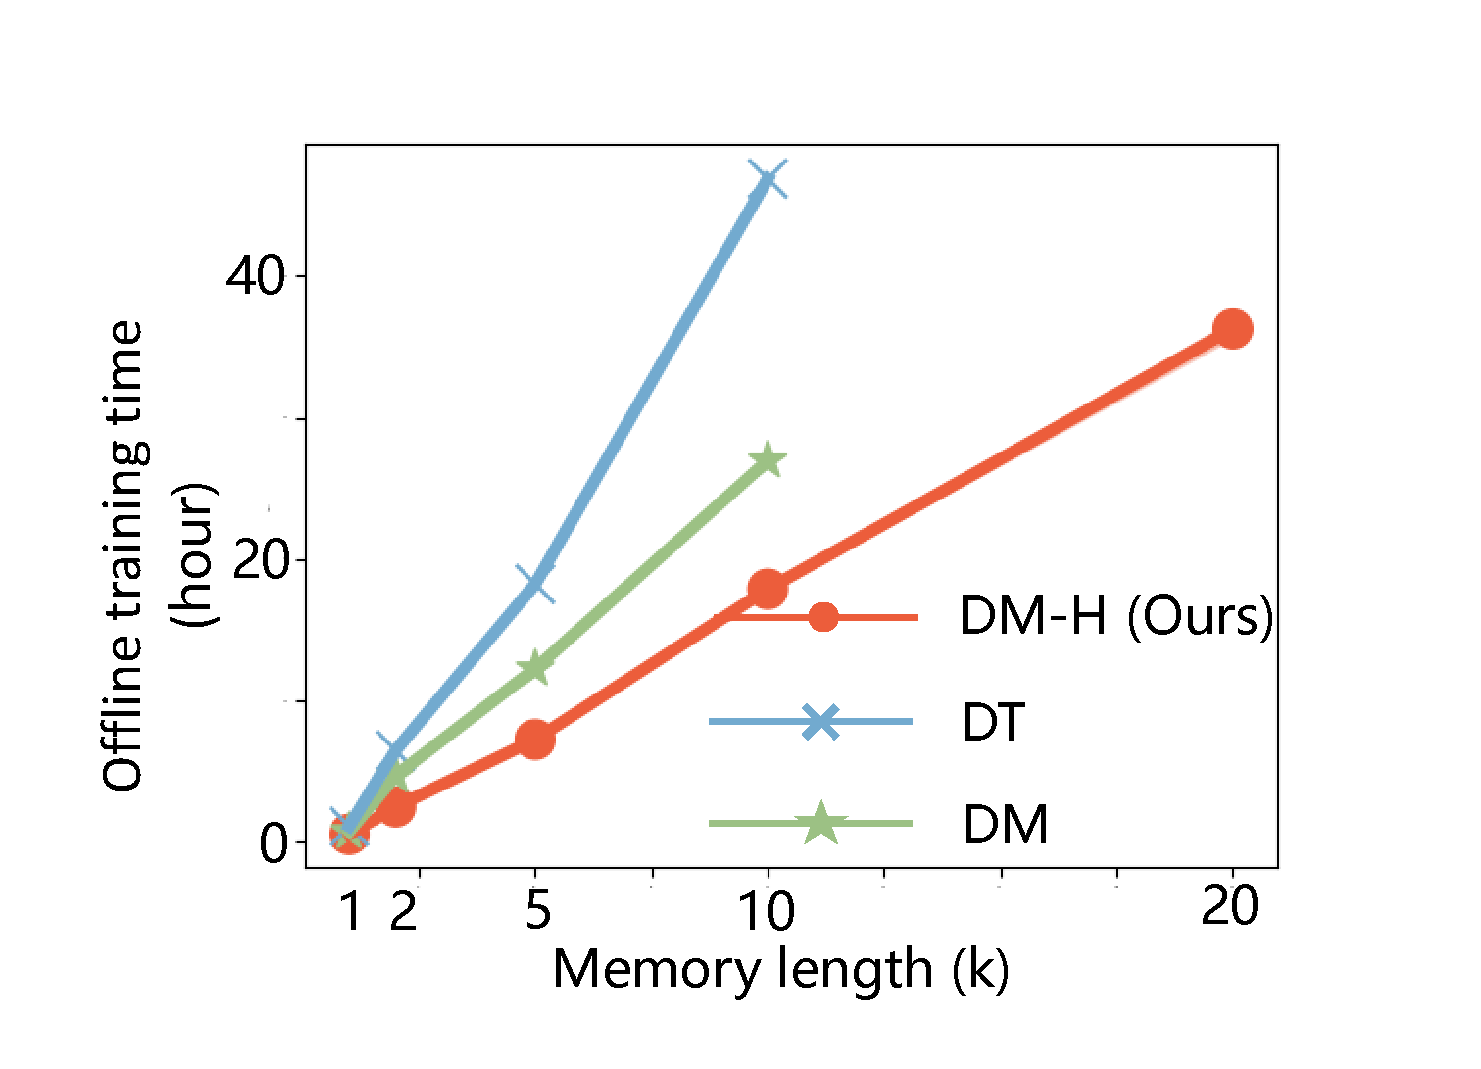
\includegraphics[width=0.5\columnwidth]{Results/Tmaze_offline.pdf}
    \caption{Results for offline training times on Tmaze tasks. We train each method to address Tmaze tasks that have different horizons until we run out of GPU memory at context length to achieve 10k (DT, DM) or 20k (DM-H). We report the training times for 10k gradient updates on Tmaze tasks.}
    \label{Tmaze appendix}
\end{figure*}

\begin{table*}
\caption{Results for offline training and online testing times. We report the offline training time per 10k gradient updates, the online testing time for 20 episodes over Grid World, and 10 episodes over D4RL. As the task length increases, the context length is forced to grow exponentially, resulting in a square increase in computational costs. In contrast, DM-H completes trial-and-error on Mamba model in sizes smaller than other baselines, significantly reducing computational costs.
}
\begin{center}
\resizebox{1.0\textwidth}{!}{
\begin{tabular}{l|l|rrr|rrr}
\toprule
\specialrule{0em}{1.0pt}{1.0pt}
\toprule
\multirow{2}{*}{Context size (step)}&\multirow{2}{*}{Tasks} & \multicolumn{3}{c|}{Offline training (hour)} & \multicolumn{3}{c}{Online testing (minute)} \\ 
\cline{3-8}
 & & AD (Mamba) & AD (Transformer) & DM-H (Ours) & AD (Mamba) & AD (Transformer) & DM-H (Ours) \\ 
 \toprule
\multirow{4}{*}{200} & Darkroom & 0.21 & 0.23 & 0.18 & 0.20 & 0.61 & 0.21 \\ % 25x10
& Darkroom Hard & 0.22 & 0.28 & 0.20 & 0.20 & 0.56 & 0.19 \\ % 25x10
& Darkroom Dynamic & 0.24 & 0.31 & 0.21 & 0.21 & 0.62 & 0.22 \\ % 25x10
& Dark Key-to-Door & 0.65 & 1.01 & 0.41 & 0.45 & 1.50 & 0.46 \\ % 50x10
\toprule
\multirow{4}{*}{2000} & Large Darkroom & 3.52 & 4.70 & 2.38 & 5.06 & 45.08 \scriptsize{(9$\times$)} & 5.12 \\ % 200x10
& Large Darkroom Hard & 4.26 & 6.69 & 2.78 & 5.61 & 44.96 \scriptsize{(7$\times$)} & 5.59 \\ % 200x10
& Large Darkroom Dynamic & 2.71 & 5.84 & 2.63 & 5.21 & 42.12 \scriptsize{(8$\times$)} & 5.36 \\ % 200x10
& Large Dark Key-to-Door & 6.87 & 18.23 & 3.16 & 5.88 & 76.79 \scriptsize{(12$\times$)} & 6.08 \\
\toprule
\multirow{3}{*}{4000} & HalfCheetah & 28.56 & 37.10 & 20.96 & 6.16 & 173.11 \scriptsize{(28$\times$)} & 6.21 \\
& Walker2d & 26.25 & 33.77 & 19.96 & 6.01 & 172.34 \scriptsize{(26$\times$)} & 6.11 \\
& Hopper & 18.15 & 22.23 & 11.52 & 6.05 & 172.92 \scriptsize{(26$\times$)} & 6.06 \\
\toprule
\specialrule{0em}{1.0pt}{1.0pt}
\toprule
\end{tabular}
}
\end{center}
\label{appendix cost}
\end{table*}



\noindent\textbf{Dateset: D4RL.}~~
D4RL \cite{13} is a commonly used offline RL benchmark, including continuous control tasks. The different dataset settings are described below.
\begin{itemize}[leftmargin=*]
    \item Medium: 1 million timesteps generated by a ``medium" policy that performs approximately one-third as well as an expert policy.
    \item Medium-Replay: 1 million timesteps collected from the replay buffer of an agent trained to the performance of a ``medium" policy.
    \item Medium-Expert: It consists of 1 million timesteps generated by the ``medium" policy and another 1 million timesteps generated by the expert policy.
\end{itemize}

\noindent\textbf{Dataset: Tmaze.}~~
The Tmaze task provides a T-shaped maze where the agent is rewarded only by reaching the end point at the last step. However, the endpoint's location is unknown; it is only told once, at an oracle early in the maze. Therefore, any policy that achieves the maximum return must be able to recall information from the first step at the final step.

\noindent\textbf{Compute.}
Experiments are carried out on NVIDIA GeForce RTX 3090 GPUs and NVIDIA A10 GPUs.
Besides, the CPU type is Intel(R) Xeon(R) Gold 6230 CPU @ 2.10GHz.
In particular, our method has lower memory requirements because it naturally shortens the across-episodic contexts.

\noindent\textbf{Hyperparameters.}
The default length of across-episodic is four trajectories unless mentioned otherwise. In D4RL, Tmaze, and Large Grid World, the transformer model generates $c=20$ steps actions while Mamba model generates one sub-goal. In conventional Grid World, we set $c=5$ because the task is too short. In summary, Table~\ref{hyper} shows the hyperparameters used in our DM-H model.

\begin{figure*}
    \centering
    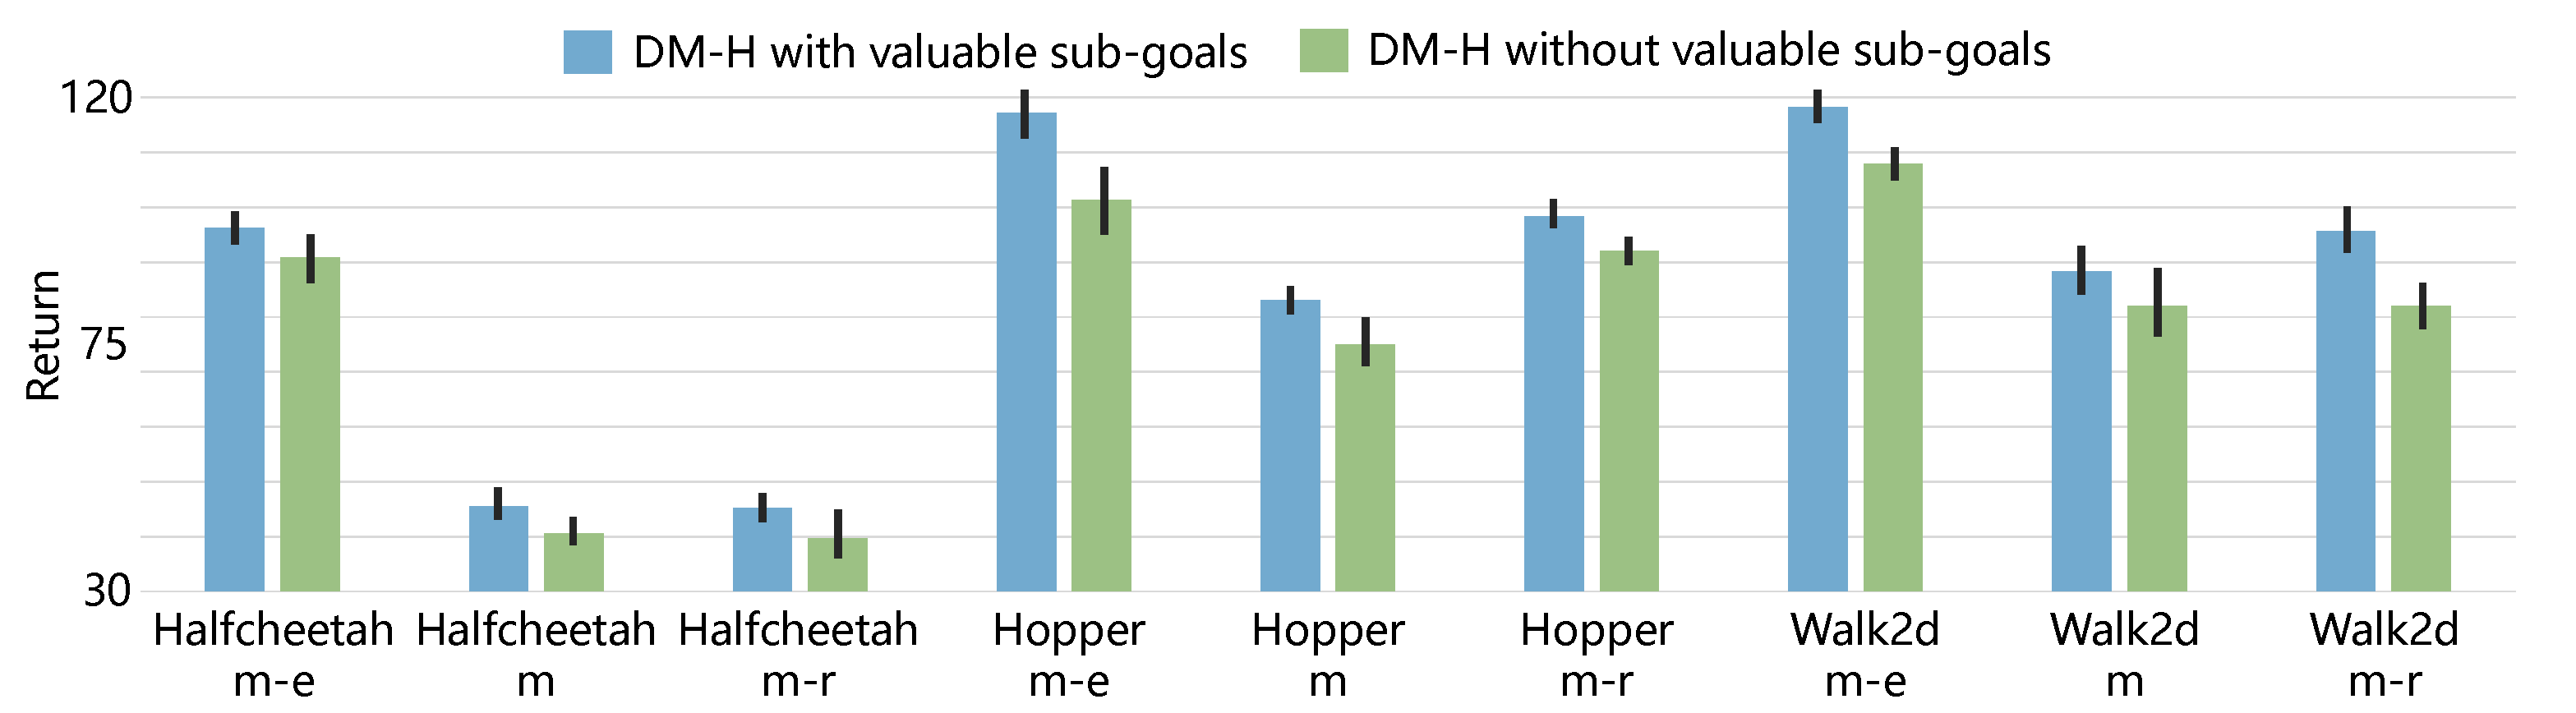
\includegraphics[width=1.0\columnwidth]{Results/Ablation_appendix.pdf}
    \caption{The ablation study on DM-H with or without valuable sub-goals.}
    \label{appendix ablation}
\end{figure*}

\section{Additional Experimental Results}
\label{additional experiments}

\noindent\textbf{Additional Tmaze Results.}~~
As described in the experiments section, we use Tmaze tasks to test the limits of DM-H's recall capabilities. We train each method to recover the optimal policy until we run out of GPU memory at a context size equal to 20k (DM-H) or 10k (DT and DM). As shown in Figure~\ref{Tmaze appendix}, DM-H achieves the maximum reward with minimum offline training costs at any task horizon. Regarding efficiency, DM-H is even faster than DM using only Mamba. This is because (1) the context of the transformer in DM-H is fixed to the hyperparameter $c$, which does not change with the task length. (2) Mamba model generates a sub-goal every $c$ steps, which shortens the sequence it processes by $c\times$ times. 

\noindent\textbf{Additional Evaluation of Computing Costs.}~~
An important property of in-context RL is that it can improve itself without expensive gradient updates during online testing. However, the computational costs of forward propagation are hidden in short-horizon tasks. Therefore, we reported the offline training time per 10k gradient updates, the online time for 20 episodes over Grid World, and 10 episodes over D4RL. As shown in Table~\ref{appendix cost}, our DM-H has efficient training and significantly reduces the online testing time compared to the baselines, approximately \textbf{28$\times$} times faster in D4RL and \textbf{12$\times$} times faster in large Grid World. As the task length increases, the online testing time of AD grows quadratically.
This is because the across-episodic contexts multiply the sequence length, leading to intolerable computational costs in the self-attention mechanism. In contrast, DM-H leverage Mamba to process long-term sequence, where the computational complexity increases linearly with length.

\noindent\textbf{Additional Ablation Study on Valuable Sub-goals.}~~
To validate the effectiveness of valuable sub-goals, we also conduct an ablation study of DM-H in D4RL tasks.
Figure~\ref{appendix ablation} presents the ablation results, which report the mean episode return across 10 seeds. We can observe that sub-goals can significantly improve DM-H's performance, proving that the sub-goal strengthens the transformer's dependency on long-term contexts from Mamba.

